% Performance and Scaling of ug4 introduction {{{
Our base code \ug is parallelized using MPI and written in C++ and has been extensively 
benchmarked elsewhere (Vogel et al., 2013; Heppner et al., 2013) and shown to scale to $>$ 200,000 processes. The solver interfaces of \ug are designed with parallel computing in mind. The first benchmark or standard test problem is the Laplace equation in three dimensional space on a unit cube. The second order elliptic partial  differential equation reads, where $\Phi$ is a scalar function in the domain $\Omega \subset \mathbf{R}^n$, and $\Delta$ is the Laplace operator:
\begin{equation}
\Delta \Phi = 0
\end{equation}

Strong scaling is demonstrated for a sevenfold regularly refined unit cube, cf.
Tab. \ref{tab:xsede_strong_scaling} and Fig. \ref{fig:speedup_laplace}. The execution time roughly halves by doubling the number of processes. A weak scaling study, cf. Tab. \ref{tab:xsede_weak_scaling} and Fig. \ref{fig:scaled_speedup_laplace}, \ref{fig:scaled_speedup_laplace2} on SDSC Comet and TACC Stampede2  confirms the scaling behavior. With each refinement of the grid the degrees of freedom (DoFs) increase by a factor of 8 and thus we increased the number of processes eightfold in each refinement step.
% }}}

% {{{ 3d Laplace problem
\begin{center}
\begin{table}[H]
\centering
\begin{tabular}{lrrr} 
\toprule
Strong scaling for first problem in \ug \\
\midrule 
\emph{DoFs} & \emph{Runtime [s]} & \emph{\# Processes} & \emph{\# Nodes}\\
\midrule 
16,974,593 & 41 &  24 & 1 \\
16,974,593 & 20 &  48 & 2 \\
16,974,593 & 14 &  72 & 3 \\
16,974,593 & 10 &  96 & 4 \\
16,974,593 &  8 & 120 & 5 \\
16,974,593 &  7 & 144 & 6 \\
16,974,593 &  5 & 168 & 7 \\
16,974,593 &  2 & 192 & 8 \\
\bottomrule
\end{tabular}
\caption{Runtimes of simulations of a \textbf{3d Laplace problem} on a fixed unit
 cube domain (seven regular refinements) with \ug on the SDSC Comet HPC cluster.
Note that each node can allocate at maximum 24 processes and the maximum number
of processes or cores per job is limited to 1728 processes in total.}
\label{tab:xsede_strong_scaling}
\end{table}
\end{center}

\begin{figure}[H]
\centering
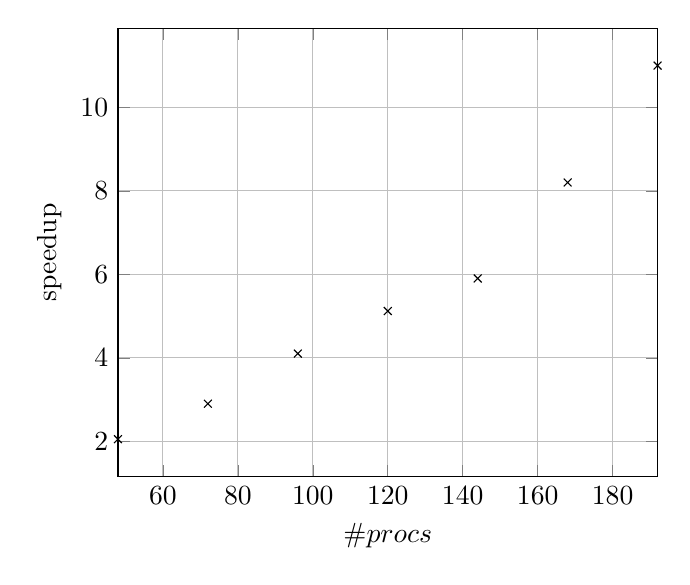
\begin{tikzpicture}
       \begin{axis}[%
            ,xlabel=$\#procs$
            ,ylabel=speedup
            ,grid=major,
            ,xmin=48,
            ,xmax=192]
            \addplot[color=black,only marks, mark=x] coordinates {(48,2.05) (72, 2.9) (96, 4.1) (120, 5.12) (144, 5.9) (168, 8.2) (192, 11)};
        \end{axis}
\end{tikzpicture}
\caption{Speedup of distributed execution. \#procs denotes the involved processes on the SDSC system Comet.}
\label{fig:speedup_laplace}
\end{figure}

\begin{center}
\begin{table}[H]
\centering
\begin{tabular}{lrrr} 
\toprule
Weak scaling for first problem in \ug \\
\midrule 
\emph{DoFs} & \emph{Runtime [s]} & \emph{\# Processes} & \emph{\# Grid refinements} \\
\midrule 
27 & 5.06 & 1 & 0 \\
216 & 5.06 & 8 & 1 \\
1,726 & 6.92 & 64 & 2 \\
13,824 & 6.92 & 512 & 3 \\
110,592 & 5.50 & 4096 & 4 \\
\bottomrule
\end{tabular}
\caption{Runtimes of simulations of a \textbf{3d Laplace problem} on a unit cube 
domain (different number of regular refinements) with \ug on the SDSC Comet HPC cluster.
Note that each grid refinement increases the DoFs by a factor 8.}
\label{tab:xsede_weak_scaling}
\end{table}
\end{center}

\begin{figure}[H]
\centering
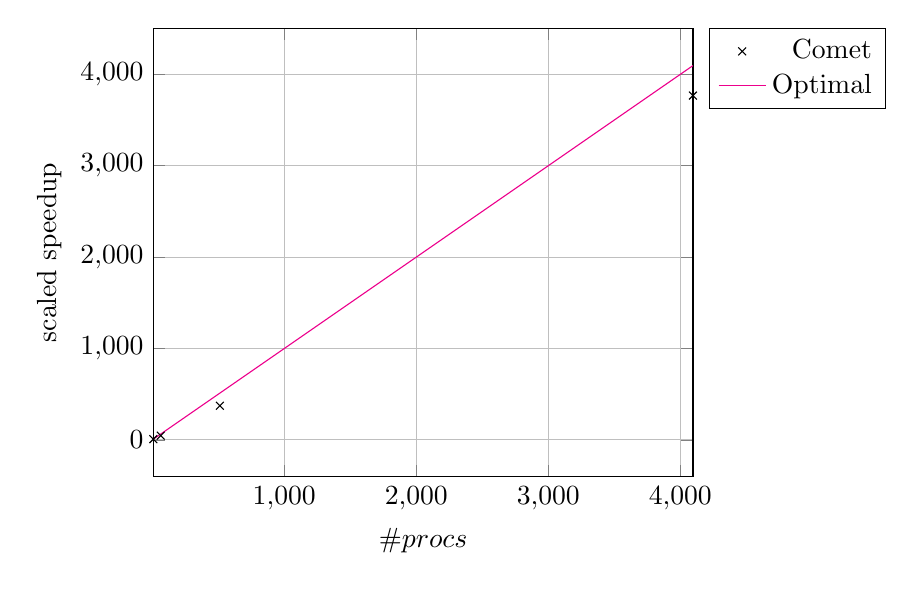
\begin{tikzpicture}
       \begin{axis}[%
            ,xlabel=$\#procs$
            ,ylabel=scaled speedup
            ,legend style={
               cells={anchor=east},
               legend pos=outer north east,
            }
            ,grid=major
            ,xmin=8,
            ,xmax=4096]
            \addplot[color=black,only marks,mark=x] coordinates {(8, 8.0) (64, 46.7) (512, 374.0) (4096, 3768.0) };
            \addplot[color=magenta] coordinates {(1,1) (4096, 4096)};
            \legend{Comet, Optimal}
        \end{axis}
\end{tikzpicture}
\caption{Scaled speedup of distributed execution. \#procs denotes the involved processes on the SDSC system Comet. Note the optimal scaling and achieved scaling behaviour of the test problem.}
\label{fig:scaled_speedup_laplace}
\end{figure}

\begin{center}
\begin{table}
\centering
\begin{tabular}{lrrr} 
\toprule
Weak scaling for first problem in \ug \\
\midrule 
\emph{DoFs} & \emph{Total runtime [s]} & \emph{\# Processes} & \emph{\# Grid refinements} \\
\midrule 
27 & 1 & 1 & 0 \\
216 & 1 & 8 & 1 \\
1,726 & 1 & 64 & 2 \\
13,824 & 1 & 512 & 3 \\
110,592 & 1 & 4096 & 4 \\
884,736 & 2 & 32768 & 5 \\
\bottomrule
\end{tabular}
\caption{Runtimes of simulations of a \textbf{3d Laplace problem} on a unit cube 
domain (different number of regular refinements) with \ug on the TACC Stampede2 HPC cluster.
Note that each grid refinement increases the DoFs by a factor of 8. Note that the \textbf{large} queue
on Stampede2 is not yet available to us to benchmark, thus we are restricted to process count up to 32768.}
\label{fig:xsede_weak_scaling}
\end{table}
\end{center}

\begin{figure}
\centering
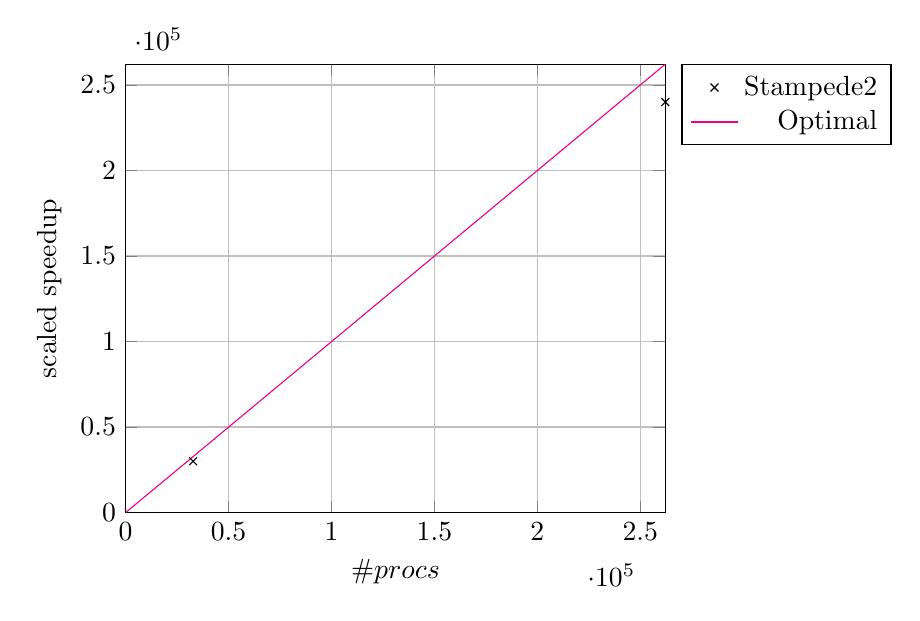
\begin{tikzpicture}
       \begin{axis}[%
            ,xlabel=$\#procs$
            ,ylabel=scaled speedup
            ,legend style={
               cells={anchor=east},
               legend pos=outer north east,
            }
            ,grid=major
            ,xmin=8,
            ,xmax=262144
            ,ymin=1
            ,ymax=262144]
            \addplot[color=black,only marks,mark=x] coordinates { (1,1) (32768, 30000) (262144, 240000)};
            \addplot[color=magenta] coordinates {(1,1) (32768, 32678) (262144, 262144) };
            \legend{Stampede2, Optimal}
        \end{axis}
\end{tikzpicture}
\caption{Scaled speedup of distributed execution. \#procs denotes the involved processes on the TACC system Stampede2. Note the optimal scaling and achieved scaling behaviour of the test problem.}
\label{fig:scaled_speedup_laplace2}
\end{figure}
% }}}

% Spine problem {{{
The second problem is motivated by neurobiology.
Of interest are the three-dimensional spatio-temporal $\textrm{Ca}^{2+}$ and $\textrm{IP}_3$ dynamics in the intracellular space of a neuron respectively spine.
This is modeled by a (system) of diffusion-reaction equations, cf. Eqns. 3-7 
in proposal.
\begin{equation}
\frac{\partial u}{\partial t} = \nabla \cdot (D \nabla u)
\end{equation}
where $u(x, t)$ stands for one of the quantities above.

\noindent The full domain equations for cytosolic calcium and calbindin are thus given by
\begin{align}
  \delT{\ccyt} & \;=\; \nabla \cdot \left( D_{c} \nabla \ccyt \right) \;+\;
    \left(\kappa_{b}^{-}\left(b^{\mathrm{tot}}-b\right)
        -\kappa_{b}^{+}\:b\:\ccyt\right), \label{eq:ccyt}\\
  \delT{b} & \;=\; \nabla \cdot \left( D_{b} \nabla b \right) \;+\;
    \left(\kappa_{b}^{-}\left(b^{\mathrm{tot}}-b\right)
        -\kappa_{b}^{+}\:b\:\ccyt\right)  \label{eq:buff}
\end{align}

 The computational grid is the reconstruction of a synaptic spine in three-dimensional space as depicted in the accompanying proposal document. Starting on the base level with a large number of DoFs the grid is refined three times. The cost for solving the problem increases only slightly but remains bound up to the testable limit, cf. scaling in Fig. \ref{fig:scaled_speedup_spine} and Tab. \ref{tab:spine_speedup}.
% {{{ 3d spine problem 
\begin{center}
\begin{table}[H]
\centering
\begin{tabular}{lrrr} 
\toprule
Weak scaling for second problem in \ug \\
\midrule 
\emph{DoFs} & \emph{Runtime [s]} & \emph{\# Processes} & \emph{\# Grid refinements} \\
\midrule 
547,348 & 37.1 & 24 & 0 \\
4,378,784 & 44 & 192 & 1 \\
35,030,272 & 57 & 1536 & 2 \\
\bottomrule
\end{tabular}
\caption{Runtime of a simulations on a \textbf{spine} reconstruction in three-dimensional
space. Note the grid has been regularly refined two times with \ug and the DoFs 
increase by a factor 8 and thus also the processes have to increase eightfold. Runtime cost
increases slightly but remains bound.}
\label{tab:spine_speedup}
\end{table}
\end{center}

\begin{figure}[H]
\centering
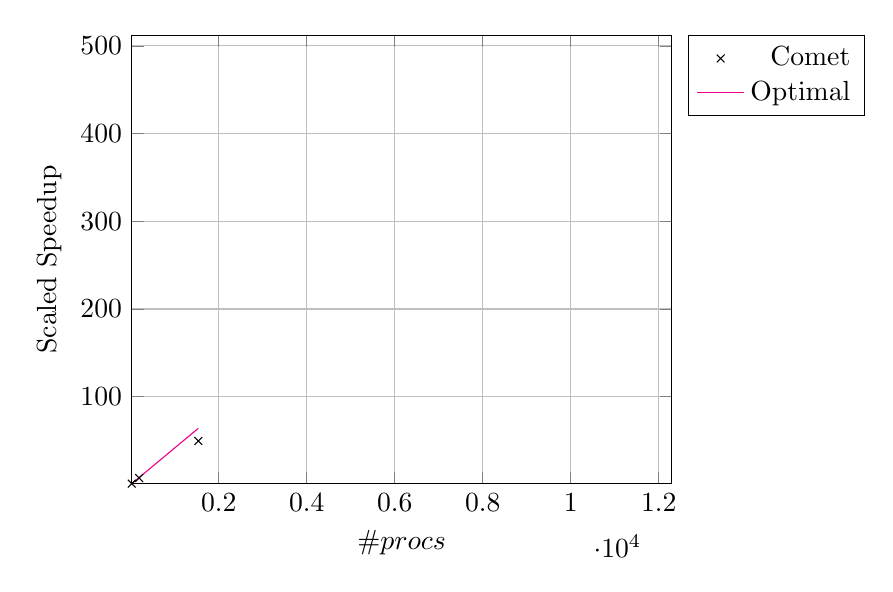
\begin{tikzpicture}
       \begin{axis}[%
            ,xlabel=$\#procs$
            ,ylabel=Scaled Speedup
            ,legend style={
               cells={anchor=east},
               legend pos=outer north east,
            }
            ,grid=major
            ,xmin=24,
            ,xmax=12288
            ,ymin=1
            ,ymax=512]
            \addplot[color=black,only marks,mark=x] coordinates {(24, 1.0) (192, 7.4) (1536, 49.6) };
            \addplot[color=magenta] coordinates {(24, 1.0) (192, 8) (1536, 64)};
            \legend{Comet, Optimal}
        \end{axis}
\end{tikzpicture}
\caption{Scaled speedup of distributed execution. \#procs denotes the involved processes on the SDSC system Comet.}
\label{fig:scaled_speedup_spine}
\end{figure}
% }}}
% }}}
